\documentclass[aspectratio=169,xcolor=dvipsnames]{beamer}
\usetheme{SimpleDarkBlue}

\usepackage{hyperref}
\usepackage{graphicx} % Allows including images
\usepackage{booktabs} % Allows the use of \toprule, \midrule and \bottomrule in tables
\usepackage{subfigure}
\usepackage{amsmath, amssymb, amscd, amsthm, amsfonts}

%----------------------------------------------------------------------------------------
%    TITLE PAGE
%----------------------------------------------------------------------------------------

\title{Wireless Networks Project Defense}
\subtitle{Zero-Forcing Beamforming for Visible Light Communication Systems}

\author{Gabriel Pereira de Carvalho}

\institute
{
	Ecole polytechnique
}
\date{March 18, 2025} % Date, can be changed to a custom date

\begin{document}
	
	\begin{frame}
		% Print the title page as the first slide
		\titlepage
	\end{frame}
	
	\begin{frame}{Overview}
		\tableofcontents
	\end{frame}
	
	\section{Introduction}
	
	\begin{frame}{Spectrum crunch problem}
		\begin{itemize}
			\item With the growth of IoT, traditional RF technologies (Wi-Fi, 4G or 5G) are experiencing more and more congestion (\textbf{Spectrum crunch}).
			\item Visible light spectrum is bigger, less congested and higher frequencies $\implies$ higher speeds (data rates $\approx 220$ gigabits per second).
		\end{itemize}
		\begin{figure}
			\centering
			\includegraphics[width = .5\textwidth]{EM_spectrum.png}
		\end{figure}
		\begin{block}{}
			Visible light spectrum used by Visible Light Communication(VLC) technologies ($400 THz$ to $800 THz$) is approximately 1000 times larger than the radio frequency spectrum ($3kHz$ to $300GHz$).
		\end{block}
	\end{frame}
	
	\begin{frame}{VLC systems}
		\begin{itemize}
			\item Visible light cannot go through walls $\implies$ indoor networks
			\item Because LED switching speed is high $\implies$ lamp can also be used for illumination.
		\end{itemize}
		\begin{figure}[h!]
			\centering
			\includegraphics[scale = 0.65]{../images/VLCscheme.PNG}
			\caption{}
		\end{figure}
	\end{frame}
	
	\begin{frame}{VLC security problems}
		\begin{itemize}
			\item Visible light $\implies$ transmissions are open and broadcasted.
			\item Photoreceptor devices in the environment can receive confidential messages!
		\end{itemize}
		\begin{figure}[h!]
			\centering
			\includegraphics[scale = 0.65]{wiretap.PNG}
		\end{figure}
		\begin{block}{Two types of eavesdropping devices}
			\begin{itemize}
				\item \textbf{Active ED:} device in direct communication with the access points.
				\item \textbf{Passive ED:} camera, smartphone or other photoreceptor not in the network.
			\end{itemize}
		\end{block}
	\end{frame}
	
	\section{Modelisation}
	
	\begin{frame}{Modelisation: Wiretap VLC system}
		\begin{itemize}
			\item \textbf{IM} (intensity modulation) and \text{DD} (direct detection demodulation) $\implies$ we are intereseted on the intensity of light that is provided by the AP and that is received by the detector in each device.
			\item $N$ APs located at its ceiling, $1$ AU, $P$ AEDs $\{ AE_1, AE_2, ..., AE_P \}$ and $Q$ randomly distributed PEDs $\{ PE_1, PE_2, ..., PE_Q \}$.
			\item We use the index $k \in \{AU, AE_p, PE_q\}$ to refer to a generic device.
		\end{itemize}
		\begin{figure}[h!]
			\centering
			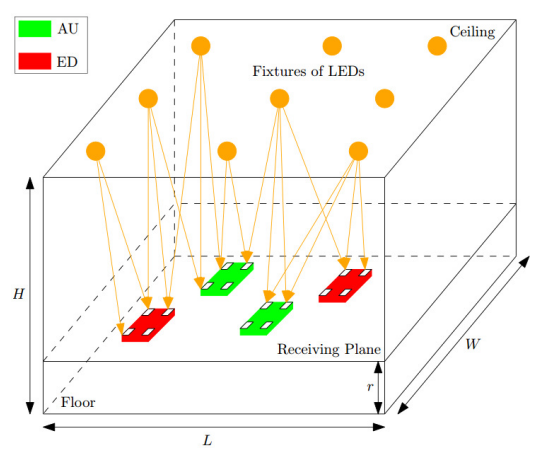
\includegraphics[scale=0.4]{../../modelisation.PNG}
		\end{figure}
	\end{frame}
	
	\begin{frame}{Zero-forcing beamforming}
		\begin{itemize}
			\item \textbf{Idea}: use interference of waves from APs to maximize signal at AU and minimize it at EDs.
			\item Our goal is to determine the beamforming vector $w = [w_1,w_2,...,w_N]^T \in \mathbb{R}^N$ where $w_i$ is a weight for the signal from the $i$-th AP.
		\end{itemize}
		\begin{figure}[h!]
			\centering
			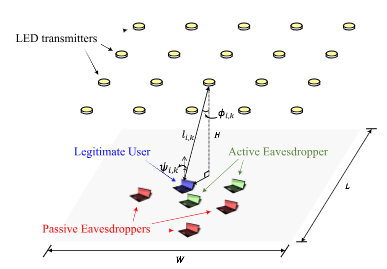
\includegraphics[scale=0.8]{../../geometry.PNG}
			\caption{Geometrical parameters in the generalized VLC model \cite{Oxford2021}}
		\end{figure}
	\end{frame}
	
	\begin{frame}{Received signal $y_k(t)$ at device $k$}
		\begin{itemize}
			\item To model the Line of Sight (LoS) gain on the path from $i$-th AP to device $k$, we use channel gain $h_{i,k} \in \mathbb{R}$.
			\begin{equation}
				y_k(t) = \alpha I_DC (h_k \cdot w) s(t) + n_k(t)
			\end{equation}
		\end{itemize}
		\begin{figure}[h!]
			\centering
			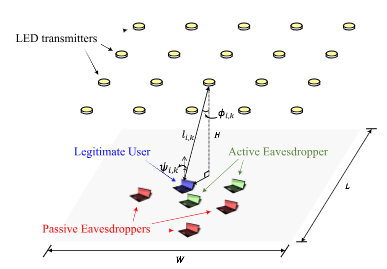
\includegraphics[scale=0.8]{../../geometry.PNG}
			\caption{Geometrical parameters in the generalized VLC model \cite{Oxford2021}}
		\end{figure}
	\end{frame}
	
	\section{Beamforming with one AED}
	
	\begin{frame}{Solving problem for one AED}
		The beamforming vector \( w \) must:
		\begin{enumerate}
			\item Maximize the received signal at the AU.
			\item Ensure that the signal received at the AED is zero.
		\end{enumerate}
		
		\begin{equation}
			h_{AED} \cdot w = 0 \implies w \in h_{AED}^\perp
		\end{equation}
		
		To maximize SNR at AU, we project $h_{AU}$ in $h_{AED}^\perp$.
		
		\begin{figure}[h!]
			\centering
			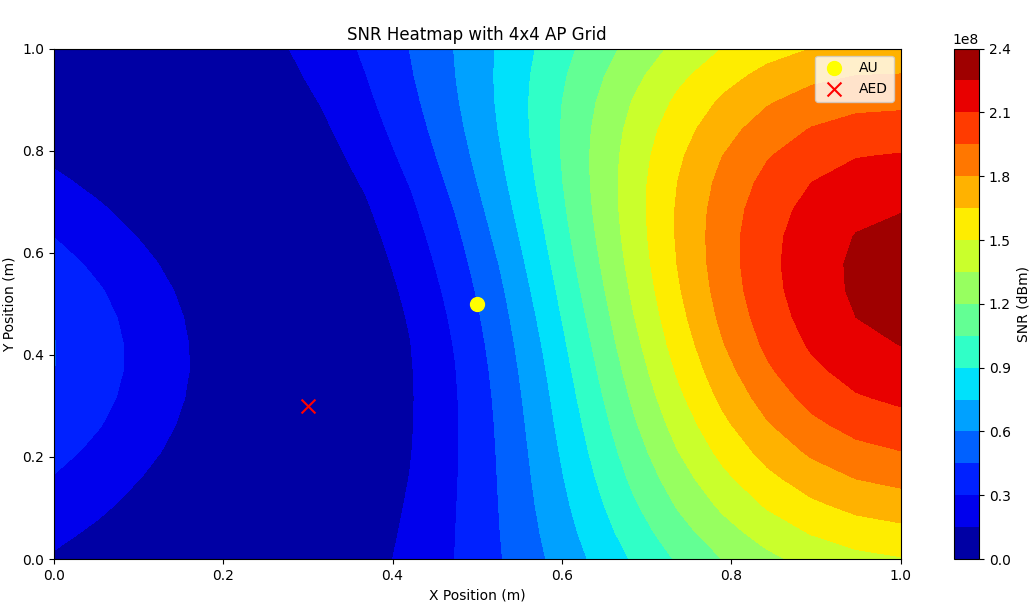
\includegraphics[width=.5\textwidth]{../../oneAED.PNG}
		\end{figure}
	\end{frame}
	
	\section{Beamforming with $P>1$ AEDs}
	
	\begin{frame}{Solving problem for $P > 1$ AEDs}
		\begin{equation}
			Y_{AED}(t) = \alpha I_DC (H_{AED} w) s(t) + N_{AED}(t) \quad \text{ with } H_{AED} =
			\begin{bmatrix}
				h_{AED_1}^T \\
				h_{AED_2}^T \\
				\vdots \\
				h_{AED_P}^T
			\end{bmatrix} 
		\end{equation}
		\begin{figure}[h!]
			\centering
			\subfigure[$N = 4$]{
				\includegraphics[width=.45\textwidth]{../../multipleAED_N4.PNG}
			}
			\hfill
			\subfigure[$N = 16$]{
				\includegraphics[width=.45\textwidth]{../../multipleAED_N16.PNG}
			}
			%\caption{SNR simulation for zero-forcing beamforming with three AEDs}
		\end{figure}
	\end{frame}
	
	\section{Beamforming with $P>1$ AEDs and PEDs}
	
	\begin{frame}{Solving problem for $P > 1$ AEDs and PEDs}
		The beamforming vector \( w \) must:
		\begin{enumerate}
			\item Maximize the received signal at the AU.
			\item Ensure that the signal received at the AED is zero.
			\item \textbf{Ensure that the peak SNR is achieved at the AU}
		\end{enumerate}
		\begin{align}
			\min_w \quad & \max_{(x,y) \in \Omega} \text{SNR}(x, y, w)  \\
			\text{s.t.} \quad & H_{AED} w = 0, \\
			& h_{AU} \cdot w = 1 \quad \text{ to ensure SNR is maximal at the AU}
		\end{align}
	\end{frame}
	
	\begin{frame}{Numerical approximation}
		\begin{itemize}
			\item Scipy offers different optimizers to solve multiple constraints optimization problems
				\begin{itemize}
					\item \texttt{SLSQP} (Sequential Least Squares)
					\item \texttt{trust-constr} (Trust Region Constrained Algorithm)
				\end{itemize}
			\item Computation time rises fast with number of APs and PEDs.
		\end{itemize}
		
		\begin{figure}[h!]
			\centering
			\includegraphics[width=.4\textwidth]{../../PEDgrid.PNG}
			\caption{Sampling of possible PED positions}
		\end{figure}
	\end{frame}
	
	\begin{frame}{Simulation results with AEDs and PEDs}
		\begin{figure}[h!]
			\centering
			\includegraphics[width=.6\textwidth]{simu2.PNG}
		\end{figure}
	\end{frame}
	
	\begin{frame}{Simulation results with AEDs and PEDs}
		\begin{figure}[h!]
			\centering
			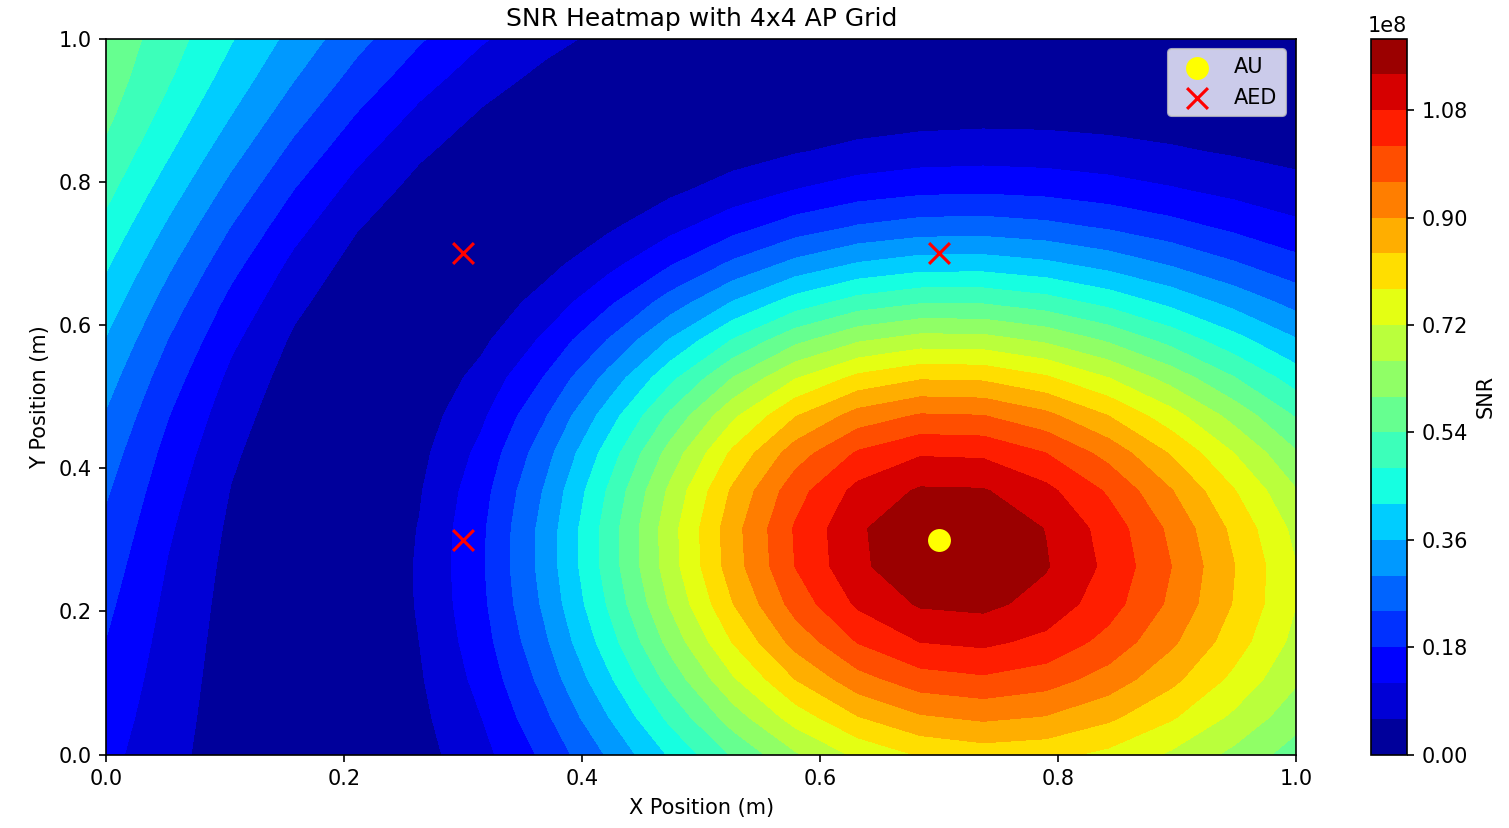
\includegraphics[width=.6\textwidth]{../../simu3.PNG}
		\end{figure}
	\end{frame}
	
	\begin{frame}
		\Huge{\centerline{\textbf{Thank you for your attention!}}}
	\end{frame}
	
\end{document}
